\documentclass[final]{beamer}
\usepackage{hyperref,xspace,graphicx,microtype,minted,multicol,mflogo,enumerate,mathtools,hologo}
\usepackage[brazil]{babel}

\usetheme[sectionpage=none,numbering=none]{metropolis}
\beamertemplatenavigationsymbolsempty

\newcommand{\filename}[1]{\texttt{#1}}
\newcommand{\code}[1]{\texttt{#1}}

\title{Introdução ao \LaTeX\ no SciELO}
\author{Rafael Beraldo}
\date{7 e 8 de junho de 2017}

\begin{document}
\maketitle
%% História %%%%%%%%%%%%%
\section{História}

\begin{frame}[plain]
  \begin{figure}[h]
    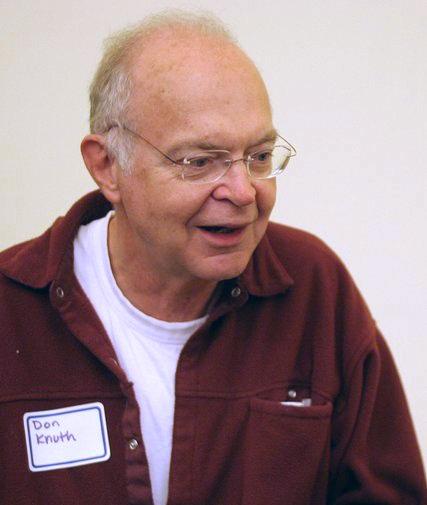
\includegraphics[scale=.5]{imagens/knuth}
    \caption{Donald Knuth em 2005}
  \end{figure}
\end{frame}

\begin{frame}[plain]
  \hspace*{-11.5mm}
  \begin{centering}
    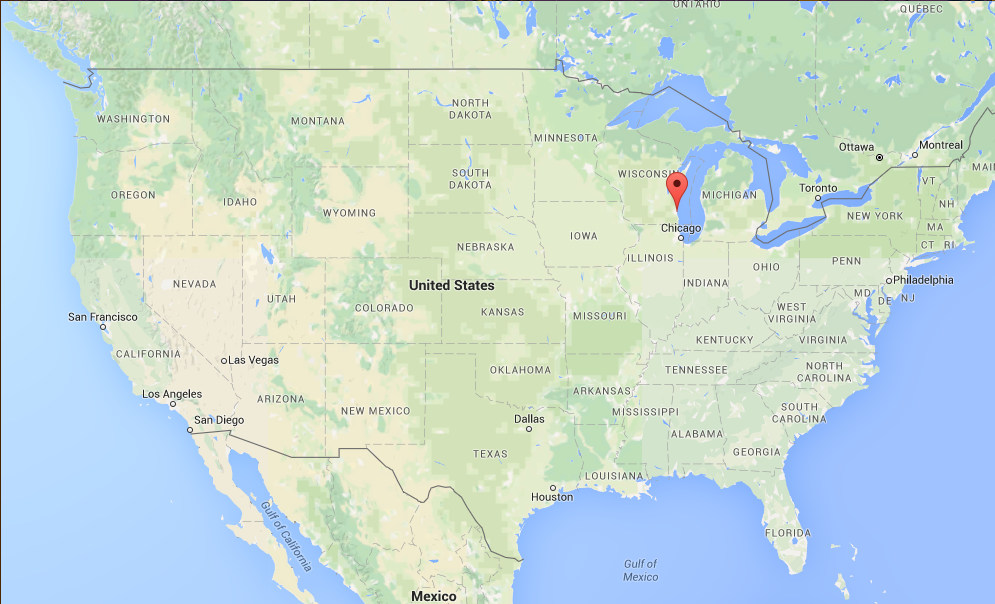
\includegraphics[width=\pagewidth]{imagens/milwaukee}
  \end{centering}
\end{frame}

\begin{frame}
  \frametitle{História do LaTeX}
  \LARGE
  \only<1>{O pai de Knuth\\ tinha uma editora}
  \only<2>{1977: segunda edição do segundo volume de \emph{The Art of Computer
  Programming}}
  \only<3>{\textsc{ascii} não foi projetado\\ com livros em mente}
  \only<4>{\TeX: tau epsilon chi}
\end{frame}

\begin{frame}
  \large
  \begin{quote}
    The purpose of this pronunciation exercise is to remind you that \TeX\ is
    primarily concerned with high-quality technical manuscripts: Its emphasis
    is on art and technology, as in the underlying Greek word. If you merely
    want to produce a passably good document—something acceptable and basically
    readable but not really beautiful—a simpler system will usually suffice.
    With \TeX\ the goal is to produce the finest quality; this requires more
    attention to detail, but you will not find it much harder to go the extra
    distance, and you’ll be able to take special pride in the finished
    product.\hfill (Donald Knuth, \emph{\TeX book})
  \end{quote}
\end{frame}

\begin{frame}
  \frametitle{História do LaTeX}
  \LARGE
  \LaTeX: 1985
\end{frame}

\begin{frame}[plain]
  \begin{figure}[h]
    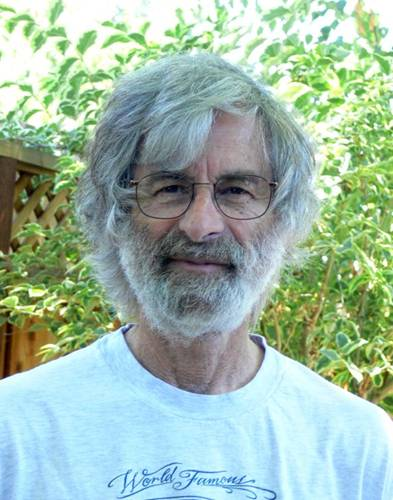
\includegraphics[scale=.5]{imagens/lamport}
    \caption{Leslie Lamport}
  \end{figure}
\end{frame}

% LaTeX: uma linguagem de marcação %%%%%%%%%%%%%%
\section[\LaTeX: uma linguagem de marcação]{Linguagem de marcação}

% O LaTeX é uma linguagem de marcação de texto, ou markup
\begin{frame}
  \frametitle{\LaTeX: uma linguagem de marcação}
  \LARGE
  \only<1>{\LaTeX{} é uma linguagem de \emph{markup}}
  \only<2>{Você \emph{declara} o documento}
  \only<3>{O programa segue as instruções}
  \only<4>{Assim como em \textsc{html},\\ o arquivo fonte é renderizado}
  \only<5>{Comandos são semânticos}
\end{frame}

% Se os comandos são semânticos, devem ser fáceis de interpretar. O que os
% comandos abaixo significam?
\begin{frame}[fragile]
  \frametitle{\LaTeX: uma linguagem de marcação}
  \begin{minted}[autogobble,fontsize=\LARGE,breaklines]{latex}
    \tableofcontents

    \section{Introdução}
  \end{minted}
\end{frame}

% Arquivos .tex não contém formatação; são texto plano.
\begin{frame}
  \frametitle{\LaTeX: uma linguagem de marcação}
  \LARGE
  \code{.tex} são arquivos de texto plano
\end{frame}

% Exemplo de artigo %%%%%%%%%%%%%%
\section{Exemplo de artigo}

% Vejamos nosso primeiro artigo em LaTeX.
\begin{frame}
  \frametitle{Exemplo de artigo}
  \Huge
  Vejamos \filename{exemplo/artigo.tex}
\end{frame}

% Comandos %%%%%%%%%%%%%%
% Sintaxe dos comandos LaTeX
\begin{frame}[standout]
  \Huge
  Comandos
\end{frame}

% Comandos simples não têm argumentos
\begin{frame}[fragile]
  \frametitle{Comandos simples}
  \begin{minted}[autogobble,fontsize=\huge,breaklines]{latex}
    \tableofcontents
  \end{minted}
\end{frame}

% Comandos simples e espaço em branco
\begin{frame}[fragile]
  \frametitle{Comandos simples e espaço em branco}
  \begin{minted}[autogobble,fontsize=\normalsize,breaklines]{latex}
    \tableofcontents Embora isso funcione, o próximo exemplo ganha mais pontos por estilo e ajuda na leitura do código. Por quê?
  \end{minted}
\end{frame}

\begin{frame}[fragile]
  \frametitle{Comandos simples e espaço em branco}
  \begin{minted}[autogobble,fontsize=\normalsize,breaklines]{latex}
    \tableofcontents
    Esse exemplo é melhor, mas como espaço em branco não faz diferença, talvez valesse a pena colocar mais uma linha entre o parágrafo e o comando.
  \end{minted}
\end{frame}

% Comandos com argumentos
\begin{frame}[fragile]
  \frametitle{Comandos com argumento}
  \begin{minted}[autogobble,fontsize=\normalsize,breaklines]{latex}
    \section{Introdução}\label{introducao}Este exemplo funciona, mas o código não é muito legível. O resultado será perfeito, entretanto.
  \end{minted}
\end{frame}

% Voltemos ao exemplo para demonstrar
\begin{frame}[standout]
  \Huge
  \filename{exemplo/artigo.tex}
\end{frame}

% Espaço em branco %%%%%%%%%%%%%%
\begin{frame}[standout]
  \Huge
  Espaço em branco
\end{frame}

% Espaços em branco são condensados
\begin{frame}[fragile]
  \frametitle{Espaços em branco}
  \begin{minted}[autogobble,fontsize=\normalsize,breaklines]{latex}
    \section      {Introdução}
        \label{introducao}

        Este exemplo funciona, mas o código não é
     muito legível.  O resultado será perfeito, entretanto.
  \end{minted}
\end{frame}

% Voltemos ao exemplo para aprender mais sobre espaços em branco e como usá-lo
% de maneira a deixar seu código mais legível.
\begin{frame}[standout]
  \Huge
  \filename{exemplo/artigo.tex}
\end{frame}

% Vamos resolver nosso primeiro exercício e compilar o arquivo. Haverá um
% problema bem claro.
\begin{frame}[standout]
  \Huge
  \filename{exercicios/espaco-branco.tex}
\end{frame}

% Símbolos especiais %%%%%%%%%%%%%%
\begin{frame}[standout]
  \Huge
  Símbolos especiais
\end{frame}

% Aspas
\begin{frame}[fragile]
  \frametitle{Aspas}
  \begin{minted}[autogobble,fontsize=\LARGE,breaklines]{latex}
    ``Devemos abrir aspas com dois acentos graves e fechar com duas aspas
    simples.''
  \end{minted}
\end{frame}

% Traços
\begin{frame}[fragile]
  \frametitle{Hífen, travessão e meia-risca}
  \begin{minted}[autogobble,fontsize=\LARGE,breaklines]{latex}
    Leve um guarda-chuva --- ouvi na rádio que pode chover entre 10h--13h.
  \end{minted}
\end{frame}

% Os símbolos a seguir são especiais e devem ser escapados:
\begin{frame}[fragile]
  \frametitle{Caracteres reservados}
  \begin{minted}[autogobble,fontsize=\LARGE,breaklines]{latex}
    # $ % ^ & _ { } ~ \

    \# \$ \% \^{} \& \_ \{ \} \~{} \textbackslash
  \end{minted}
\end{frame}

% Resolver o exercício
\begin{frame}[standout]
  \Huge
  \filename{exercicios/caracteres\-reservados.tex}
\end{frame}

%
% pacotes.tex
%
% Rafael Beraldo <rberaldo@cabaladada.org>
% Workshop de LaTeX do SciELO
%
% Problema: ao compilar este documento, os acentos não aparecem no PDF.
% Adicione o pacote polyglossia após a linha 13, configure o idioma português e
% compile.
%

\documentclass{article}
\begin{document}
  Muito além, nos confins inexplorados da região mais brega da
  Borda Ocidental desta Galáxia, há um pequeno sol amarelo e esquecido.

  Girando em torno deste sol, a uma distância de cerca de 148~milhões de
  quilômetros, há um planetinha verde-azulado absolutamente insignificante.
\end{document}

\begin{frame}[standout]
  \Huge
  Obrigado!
\end{frame}

\begin{frame}
  \begin{center}
    \vspace{2em}
    
\includegraphics[width=3cm]{imagens/cc}\\
    2016 Alguns direitos reservados para Rafael Beraldo
    \vspace{1em}
    \url{http://creativecommons.org/licenses/by-sa/4.0/}
    \vfill
    \huge{Powered by \LaTeX{}}
  \end{center}
\end{frame}

\end{document}
